\makeatletter
\def\input@path{{./}{../../../preamble/}{book2026-2027/preamble/}}
\makeatother
\input{preamble.tex}
\usepackage{needspace}
\hypersetup{pdftitle={Grade 10 Term 2 Discrete Probability}}
\setlength{\emergencystretch}{2em}
\title{Grade 10, Term 2, Lesson 1, Criterion C2\\Reading and Checking PMFs and CDFs}
\author{}
\date{}
\begin{document}
\maketitle
\setcounter{tocdepth}{1}
\setcounter{secnumdepth}{2}
\phantomsection\label{toc}
\tableofcontents
\section*{Evaluated criterion}
\textbf{C2:} Interprets PMFs and CDFs by verifying their defining properties and using them to calculate point, interval, cumulative, and complementary probabilities in financial contexts.
\section{Introduction}\label{sec:t2-c2-introduction}
All data in this activity are hypothetical teaching models. Probabilities have no monetary units. Keep exact expressions where useful and round final probabilities to four decimal places.
\subsection{Individual and accumulated probabilities}
A school shop counts refunds in an afternoon. Exactly two means one value; at most two includes zero, one and two. The PMF $p_X(x)=P(X=x)$ is read as the probability that X equals x. The CDF $F_X(x)=P(X\leq x)$ is read as the probability that X is at most x. Capital $X$ names the random variable, while $x$ is a value or cutoff. Refund counts have units of refunds; probabilities have no units.
\textbf{Check.} Does $F_X(2)$ mean exactly two? \emph{Suggested answer:} No. It adds all mass at values at most 2.


\subsection{Defining properties}
A PMF is non-negative and its masses total 1. A CDF is non-decreasing: raising the cutoff cannot remove outcomes. It is right-continuous: the value at a jump equals the height immediately to its right. Its limits are 0 as $x\to-\infty$ and 1 as $x\to+\infty$, meaning arbitrarily far left and right. For finite discrete support, it is constant between supported values and jumps by $p_X(x)$ at each value.
\textbf{Check.} May a CDF decrease from 0.7 to 0.5? \emph{Suggested answer:} No. Cumulative probability cannot decrease.


\subsection{Endpoints}
At most means $\leq$; less than means $<$; at least means $\geq$; more than means $>$. For integer counts $P(X<3)=F_X(2)$, but for irregular support list the actual included values. A CDF accepts all real cutoffs, including values outside the support.
\textbf{Check.} For support $\{0,2,5\}$, what does $1<X<5$ contain? \emph{Suggested answer:} Only $X=2$.

\textbf{Check.} What is the complement of $X>2$? \emph{Suggested answer:} $X\leq2$, so $P(X>2)=1-F_X(2)$.

\section{General worked problems}
\Needspace{14\baselineskip}
\subsection{Introductory general problem: PMF to CDF}
A score $X$ has support $\{0,2,5\}$ and masses $0.2,0.5,0.3$.

\textbf{Questions/Tasks}
\begin{enumerate}
\item Verify the PMF; construct the complete CDF and graphs; find $P(0<X\leq5)$ and $P(X<5)$.
\end{enumerate}
\subsubsection*{Complete worked solution}
\begin{center}
\begin{tabular}{llp{0.48\linewidth}}
\toprule
Symbol & Value & Meaning in this problem \\ \midrule
$X$ & $0,2,5$ & Supported score values \\
$p_X(x)$ & $0.2,0.5,0.3$ & Respective masses; no units \\
\bottomrule
\end{tabular}
\end{center}

\par\noindent\begin{minipage}{\linewidth}
\textbf{Step 1: Define and validate.} $X$ is a score. Its masses are positive and $0.2+0.5+0.3=1$, so the table is valid; no independent-trials model is required.
\end{minipage}\par\medskip
\par\noindent\begin{minipage}{\linewidth}
\textbf{Step 2: Accumulate.} $F_X(x)=\sum_{u\leq x}p_X(u)$. The summation sign means add masses at supported values $u$ at most the cutoff $x$.\[F_X(x)=\begin{cases}0,&x<0,\\0.2,&0\leq x<2,\\0.7,&2\leq x<5,\\1,&x\geq 5.\end{cases}\]
\begin{center}
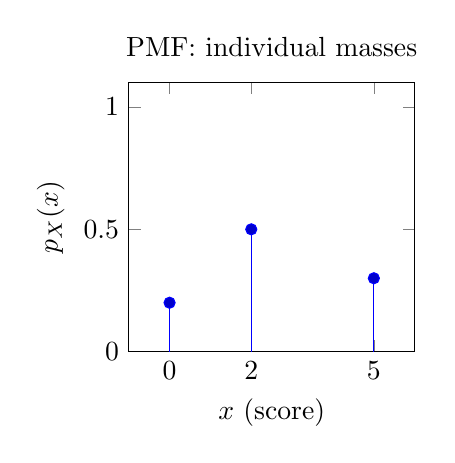
\begin{tikzpicture}
\begin{axis}[width=0.43\linewidth,height=5cm,xmin=-1,xmax=6,ymin=0,ymax=1.1,xtick={0,2,5},xlabel={$x$ (score)},ylabel={$p_X(x)$},title={PMF: individual masses}]
\addplot+[ycomb,mark=*] coordinates {(0,0.2)(2,0.5)(5,0.3)};
\end{axis}\end{tikzpicture}\hfill
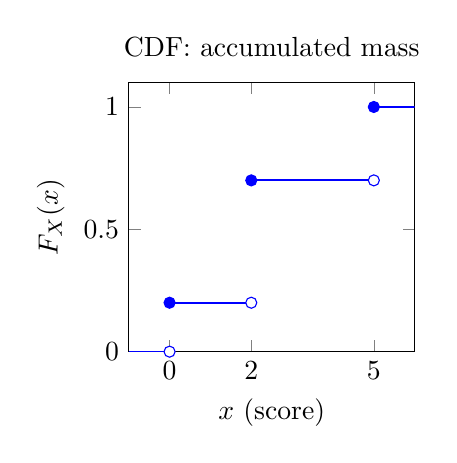
\begin{tikzpicture}
\begin{axis}[width=0.43\linewidth,height=5cm,xmin=-1,xmax=6,ymin=0,ymax=1.1,xtick={0,2,5},xlabel={$x$ (score)},ylabel={$F_X(x)$},title={CDF: accumulated mass}]
\addplot[blue,thick] coordinates {(-1,0)(0,0)};
\addplot[blue,thick] coordinates {(0,0.2)(2,0.2)};
\addplot[blue,thick] coordinates {(2,0.7)(5,0.7)};
\addplot[blue,thick] coordinates {(5,1)(6,1)};
\addplot[only marks,mark=*,blue] coordinates {(0,0.2)(2,0.7)(5,1)};
\addplot[only marks,mark=*,mark options={fill=white},blue] coordinates {(0,0)(2,0.2)(5,0.7)};
\end{axis}\end{tikzpicture}\end{center}
Filled dots give included endpoint values; open dots exclude them. Each jump matches a PMF stem. Horizontal tails continue to either side.

\end{minipage}\par\medskip
\par\noindent\begin{minipage}{\linewidth}
\textbf{Step 3: Calculate.} $P(0<X\leq5)=p_X(2)+p_X(5)=0.5+0.3=0.8000$. Also $P(X<5)=p_X(0)+p_X(2)=0.2+0.5=0.7000$, whereas $F_X(5)=1$.
\end{minipage}\par\medskip
\par\noindent\begin{minipage}{\linewidth}
\textbf{Step 4: Check and interpret.} The CDF is non-decreasing, right-continuous and has limits 0 and 1. The strict upper endpoint excludes the 0.3 mass at 5.
\end{minipage}\par\medskip
\subsection{Bridge to the general model}
Write $F_X(a^-)=P(X<a)$, read as F just to the left of a. Then
\[P(X=a)=F_X(a)-F_X(a^-),\qquad P(a<X\leq b)=F_X(b)-F_X(a).\]
For an inclusive lower endpoint, $P(a\leq X\leq b)=F_X(b)-F_X(a^-)$. Also $P(X>a)=1-F_X(a)$. These identities work for irregular supports as well as consecutive integers.
\Needspace{14\baselineskip}
\subsection{Advanced general problem: recovering jumps and testing candidates}
Candidate $H$ is 0 for $x<-1$, 0.25 for $-1\leq x<1$, 0.6 for $1\leq x<4$, and 1 for $x\geq4$. Candidate $J$ agrees except $J(1)=0.25$. Candidate $K$ has successive heights $0,0.7,0.6,1$ on the same intervals.

\textbf{Questions/Tasks}
\begin{enumerate}
\item Validate each; recover the PMF of $H$ and calculate $P(-1<X\leq4)$ and $P(X\geq1)$.
\end{enumerate}
\subsubsection*{Complete worked solution}
\par\noindent\begin{minipage}{\linewidth}
\textbf{Step 1: Define and test.} $X$ is a score. $H$ has increasing heights, right-continuous endpoints and limits 0 and 1. $J$ fails right-continuity at 1: its value 0.25 differs from height 0.6 immediately to its right. $K$ decreases from 0.7 to 0.6, so it is invalid.
\end{minipage}\par\medskip
\par\noindent\begin{minipage}{\linewidth}
\textbf{Step 2: Recover the PMF.} $p_X(x)=H(x)-H(x^-)$ gives $0.25-0=0.25$, $0.6-0.25=0.35$, $1-0.6=0.4$ on support $\{-1,1,4\}$.
\end{minipage}\par\medskip
\par\noindent\begin{minipage}{\linewidth}
\textbf{Step 3: Calculate.} $P(-1<X\leq4)=H(4)-H(-1)=1-0.25=0.7500$; $P(X\geq1)=1-H(1^-)=1-0.25=0.7500$.
\end{minipage}\par\medskip
\par\noindent\begin{minipage}{\linewidth}
\textbf{Step 4: Check and interpret.} The recovered positive masses total 1. Both events contain precisely 1 and 4; their equal probabilities follow from the support.
\end{minipage}\par\medskip
\section{Notation reference and practice procedure}
\begin{center}
\begin{tabular}{lp{0.72\linewidth}}
\toprule
Symbol & Meaning and units \\ \midrule
$p_X(x)$ & $P(X=x)$: one value \\
$F_X(x)$ & $P(X\leq x)$: accumulated mass \\
$F_X(a^-)$ & $P(X<a)$: height before the jump \\
$1-F_X(a)$ & $P(X>a)$ \\
\bottomrule
\end{tabular}
\end{center}
\begin{enumerate}
\item Define the random variable in words and give its units and support.
\item List parameters and check that the model assumptions match the situation.
\item Translate ordinary language into an event, paying attention to endpoints.
\item Write the symbolic formula first, then substitute without rounding intermediate values.
\item Check bounds, total probability or a complementary calculation; interpret the answer in context.
\end{enumerate}
\Needspace{19\baselineskip}
\section{Foundational contextual practice}\label{sec:t2-c2-foundational}
\Needspace{14\baselineskip}
\subsection{Afternoon refunds}
$X$ counts refunds with masses $0.5,0.3,0.2$ at $0,1,2$.

\textbf{Questions/Tasks}
\begin{enumerate}
\item Verify the distribution, give its complete CDF and find $P(X=1)$ and $P(X\leq1)$.
\end{enumerate}
\subsubsection*{Complete worked solution}
\par\noindent\begin{minipage}{\linewidth}
\textbf{Step 1: Define and check.} $X$ counts refunds per afternoon; support $\{0,1,2\}$. The positive masses total $0.5+0.3+0.2=1$.
\end{minipage}\par\medskip
\par\noindent\begin{minipage}{\linewidth}
\textbf{Step 2: Construct.} $F_X(x)=\sum_{u\leq x}p_X(u)$ gives\[F_X(x)=\begin{cases}0,&x<0,\\0.5,&0\leq x<1,\\0.8,&1\leq x<2,\\1,&x\geq 2.\end{cases}\]

\end{minipage}\par\medskip
\par\noindent\begin{minipage}{\linewidth}
\textbf{Step 3: Calculate.} $P(X=1)=p_X(1)=0.3000$; $P(X\leq1)=p_X(0)+p_X(1)=0.5+0.3=0.8000$.
\end{minipage}\par\medskip
\par\noindent\begin{minipage}{\linewidth}
\textbf{Step 4: Check and interpret.} The CDF has non-negative jumps, right-continuous endpoints and correct tails. At most one includes zero; exactly one does not.
\end{minipage}\par\medskip
\secInicio[][sec:t2-c2-foundational]
\Needspace{14\baselineskip}
\subsection{Transaction fees}
A fee $Y$ is $0,2,5$ USD with probabilities $0.4,0.35,0.25$.

\textbf{Questions/Tasks}
\begin{enumerate}
\item Find $P(Y<2)$, $P(Y\leq2)$ and $P(1<Y<5)$.
\end{enumerate}
\subsubsection*{Complete worked solution}
\par\noindent\begin{minipage}{\linewidth}
\textbf{Step 1: Define and validate.} $Y$ is a fee in USD; support $\{0,2,5\}$. Its positive masses total $0.4+0.35+0.25=1$.
\end{minipage}\par\medskip
\par\noindent\begin{minipage}{\linewidth}
\textbf{Step 2: Translate.} The events contain respectively $\{0\}$, $\{0,2\}$ and $\{2\}$.
\end{minipage}\par\medskip
\par\noindent\begin{minipage}{\linewidth}
\textbf{Step 3: Calculate.} $P(Y<2)=p_Y(0)=0.4000$; $P(Y\leq2)=p_Y(0)+p_Y(2)=0.4+0.35=0.7500$; $P(1<Y<5)=p_Y(2)=0.3500$.
\end{minipage}\par\medskip
\par\noindent\begin{minipage}{\linewidth}
\textbf{Step 4: Check and interpret.} The first two answers differ by the 0.35 jump at 2 USD. A cutoff need not be a supported fee.
\end{minipage}\par\medskip
\secInicio[][sec:t2-c2-foundational]
\Needspace{19\baselineskip}
\section{Intermediate contextual practice}\label{sec:t2-c2-intermediate}
\Needspace{14\baselineskip}
\subsection{Late-payment counts}
A weekly count has CDF 0 for $x<0$, 0.6 for $0\leq x<2$, 0.9 for $2\leq x<3$, and 1 for $x\geq3$.

\textbf{Questions/Tasks}
\begin{enumerate}
\item Recover its PMF and find $P(X>0)$ and $P(0<X\leq2)$.
\end{enumerate}
\subsubsection*{Complete worked solution}
\par\noindent\begin{minipage}{\linewidth}
\textbf{Step 1: Define and check.} $X$ counts late payments; jumps give support $\{0,2,3\}$. The CDF is non-decreasing, right-continuous and has limits 0 and 1.
\end{minipage}\par\medskip
\par\noindent\begin{minipage}{\linewidth}
\textbf{Step 2: Recover.} $p_X(x)=F_X(x)-F_X(x^-)$ gives $0.6$, $0.9-0.6=0.3$, $1-0.9=0.1$; these positive masses total 1.
\end{minipage}\par\medskip
\par\noindent\begin{minipage}{\linewidth}
\textbf{Step 3: Calculate.} $P(X>0)=1-F_X(0)=1-0.6=0.4000$; $P(0<X\leq2)=F_X(2)-F_X(0)=0.9-0.6=0.3000$.
\end{minipage}\par\medskip
\par\noindent\begin{minipage}{\linewidth}
\textbf{Step 4: Interpret.} The first event includes 2 and 3; the second includes only 2. The plateau before 2 shows that 1 has no mass in this simplified model.
\end{minipage}\par\medskip
\secInicio[][sec:t2-c2-intermediate]
\Needspace{14\baselineskip}
\subsection{Investment gain intervals}
$G$ takes $-10,0,15,40$ USD with masses $0.2,0.3,0.4,0.1$.

\textbf{Questions/Tasks}
\begin{enumerate}
\item Find the probabilities of a loss, a positive gain, $0\leq G<40$, and the value $F_G(14)$.
\end{enumerate}
\subsubsection*{Complete worked solution}
\par\noindent\begin{minipage}{\linewidth}
\textbf{Step 1: Define and validate.} $G$ is net gain in USD; the four positive masses total 1. Its support is the four listed monetary values.
\end{minipage}\par\medskip
\par\noindent\begin{minipage}{\linewidth}
\textbf{Step 2: Translate.} Loss is $G<0$; positive gain is $G>0$. The interval contains 0 and 15.
\end{minipage}\par\medskip
\par\noindent\begin{minipage}{\linewidth}
\textbf{Step 3: Calculate.} $P(G<0)=p_G(-10)=0.2000$; $P(G>0)=1-F_G(0)=1-(0.2+0.3)=0.5000$; $P(0\leq G<40)=p_G(0)+p_G(15)=0.3+0.4=0.7000$.
\end{minipage}\par\medskip
\par\noindent\begin{minipage}{\linewidth}
\textbf{Step 4: Check and interpret.} $F_G(14)=p_G(-10)+p_G(0)=0.5000$. Positive and non-negative gain differ by the mass at zero.
\end{minipage}\par\medskip
\secInicio[][sec:t2-c2-intermediate]
\Needspace{19\baselineskip}
\section{Advanced contextual practice}\label{sec:t2-c2-advanced}
\Needspace{14\baselineskip}
\subsection{Insurance PMF audit}
Candidate A has masses $0.6,0.5,-0.1$ at counts $0,1,2$; B has $0.2,0.3,0.3$. The corrected model is $0.6,0.3,0.1$.

\textbf{Questions/Tasks}
\begin{enumerate}
\item Reject A and B; find $P(X\geq1)$ and $P(X<2)$ for the correction.
\end{enumerate}
\subsubsection*{Complete worked solution}
\par\noindent\begin{minipage}{\linewidth}
\textbf{Step 1: Define and audit.} $X$ counts daily claims with corrected support $\{0,1,2\}$. A totals 1 but contains a negative mass; B is non-negative but totals 0.8. Both are invalid.
\end{minipage}\par\medskip
\par\noindent\begin{minipage}{\linewidth}
\textbf{Step 2: Validate.} The correction is positive and totals $0.6+0.3+0.1=1$. Its CDF heights are $0,0.6,0.9,1$ on boundaries 0, 1, 2, with closed left endpoints.
\end{minipage}\par\medskip
\par\noindent\begin{minipage}{\linewidth}
\textbf{Step 3: Calculate.} $P(X\geq1)=1-P(X<1)=1-p_X(0)=1-0.6=0.4000$; $P(X<2)=p_X(0)+p_X(1)=0.6+0.3=0.9000$.
\end{minipage}\par\medskip
\par\noindent\begin{minipage}{\linewidth}
\textbf{Step 4: Check and interpret.} The complement of at least one is zero. A total of 1 alone does not establish a PMF.
\end{minipage}\par\medskip
\secInicio[][sec:t2-c2-advanced]
\Needspace{30\baselineskip}
\subsection{Account-fee CDF audit}
Fees can only be 0 or 3 USD. Candidate $H$ is 0 for $y<0$, 0.4 for $0\leq y<3$, and 0.9 for $y\geq3$. Another has heights 0, 0.4, 1 on these intervals but assigns value 0 at $y=0$.

\textbf{Questions/Tasks}
\begin{enumerate}
\item Explain both defects, construct a valid CDF retaining mass 0.4 at zero, and find $P(0<Y\leq3)$.
\end{enumerate}
\subsubsection*{Complete worked solution}
\par\noindent\begin{minipage}{\linewidth}
\textbf{Step 1: Define and diagnose.} $Y$ measures fee in USD. $H$ has limit 0.9 instead of 1 at positive infinity. The other fails right-continuity at zero.
\end{minipage}\par\medskip
\par\noindent\begin{minipage}{\linewidth}
\textbf{Step 2: Repair.} $p_Y(3)=1-p_Y(0)=1-0.4=0.6$. \[F_Y(y)=\begin{cases}0,&y<0,\\0.4,&0\leq y<3,\\1,&y\geq3.\end{cases}\]
\end{minipage}\par\medskip
\par\noindent\begin{minipage}{\linewidth}
\textbf{Step 3: Calculate.} $P(0<Y\leq3)=F_Y(3)-F_Y(0)=1-0.4=0.6000$.
\end{minipage}\par\medskip
\par\noindent\begin{minipage}{\linewidth}
\textbf{Step 4: Check and interpret.} The repaired CDF is non-decreasing, right-continuous and has limits 0 and 1. Its jumps total 1; the event is precisely a 3 USD fee.
\end{minipage}\par\medskip
\secInicio[][sec:t2-c2-advanced]
\section{Closing reference: key ideas and common errors}
A PMF assigns individual masses; a CDF accumulates them. Check non-negativity, total mass, monotonicity, right-continuity and limits. Use actual support for endpoints. Jumps give masses; plateaus add none. In $1-F_X(a)$ equality at $a$ is excluded.
\secInicio
\end{document}
